%%%%%%%%%%%%%%%%%%%%%%%%%%%%%%%%%%%%%%%%%%%%%%%%%%%%%%%%%%%%%%%%%%%%%%%%%
 
 \begin{center}
\begin{figure}[p]
\begin{tabular}{cc}
  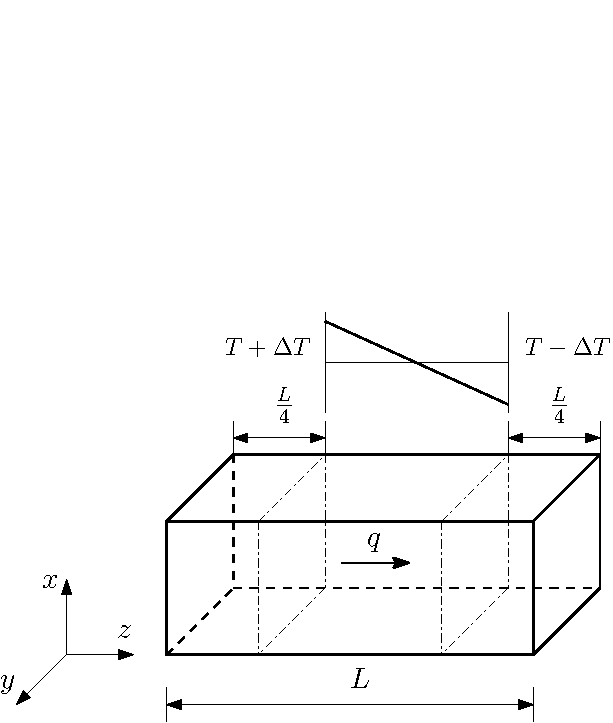
\includegraphics[width=0.48\textwidth]{./Figures/schematic}
  &
  \hspace{3mm}
  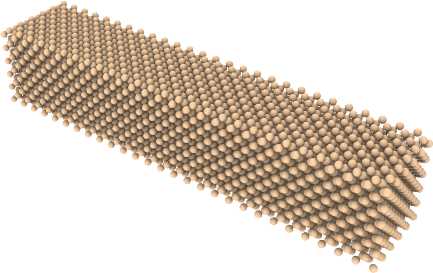
\includegraphics[width=0.40\textwidth]{./Figures/Sibar_05}
  \\ (a) & (b)
  \end{tabular}
\caption{(a) Schematic illustration of the set-up for evaluating thermal conductivity of Si using NEMD. (b) 
Arrangement of Si atoms prior to the application of thermal gradient.}
\label{fig:setup}
\end{figure}
\end{center}

\clearpage

%%%%%%%%%%%%%%%%%%%%%%%%%%%%%%%%%%%%%%%%%%%%%%%%%%%%%%%%%%%%%%%%%%%%%%%%%

